\section{Background}\label{sec:background}
\subsection{Data Normalization}\label{sec:data_normalization}
As previously mentioned, the \gls{chemcam} instrument consists of three spectrometers, each producing 2048 channels.
For data normalization, we follow the approach taken by the SuperCam team and normalize across individual spectrometers' wavelength ranges, a process known as \textit{Norm 3}~\cite{andersonPostlandingMajorElement2022}.
This method ensures that the wavelength intensities captured by each spectrometer is normalized independently.

Figure~\ref{fig:spectral_plot} shows a spectral plot of the \gls{ccs} data for the \textit{ultramafic} sample, illustrating the three distinct spectral regions, each captured by one of the three spectrometers. Specifically, one spectrometer captures the \gls{uv} region, another captures the \gls{vio} region, and the third captures the \gls{vnir} region.

\begin{figure}[H]
	\centering
	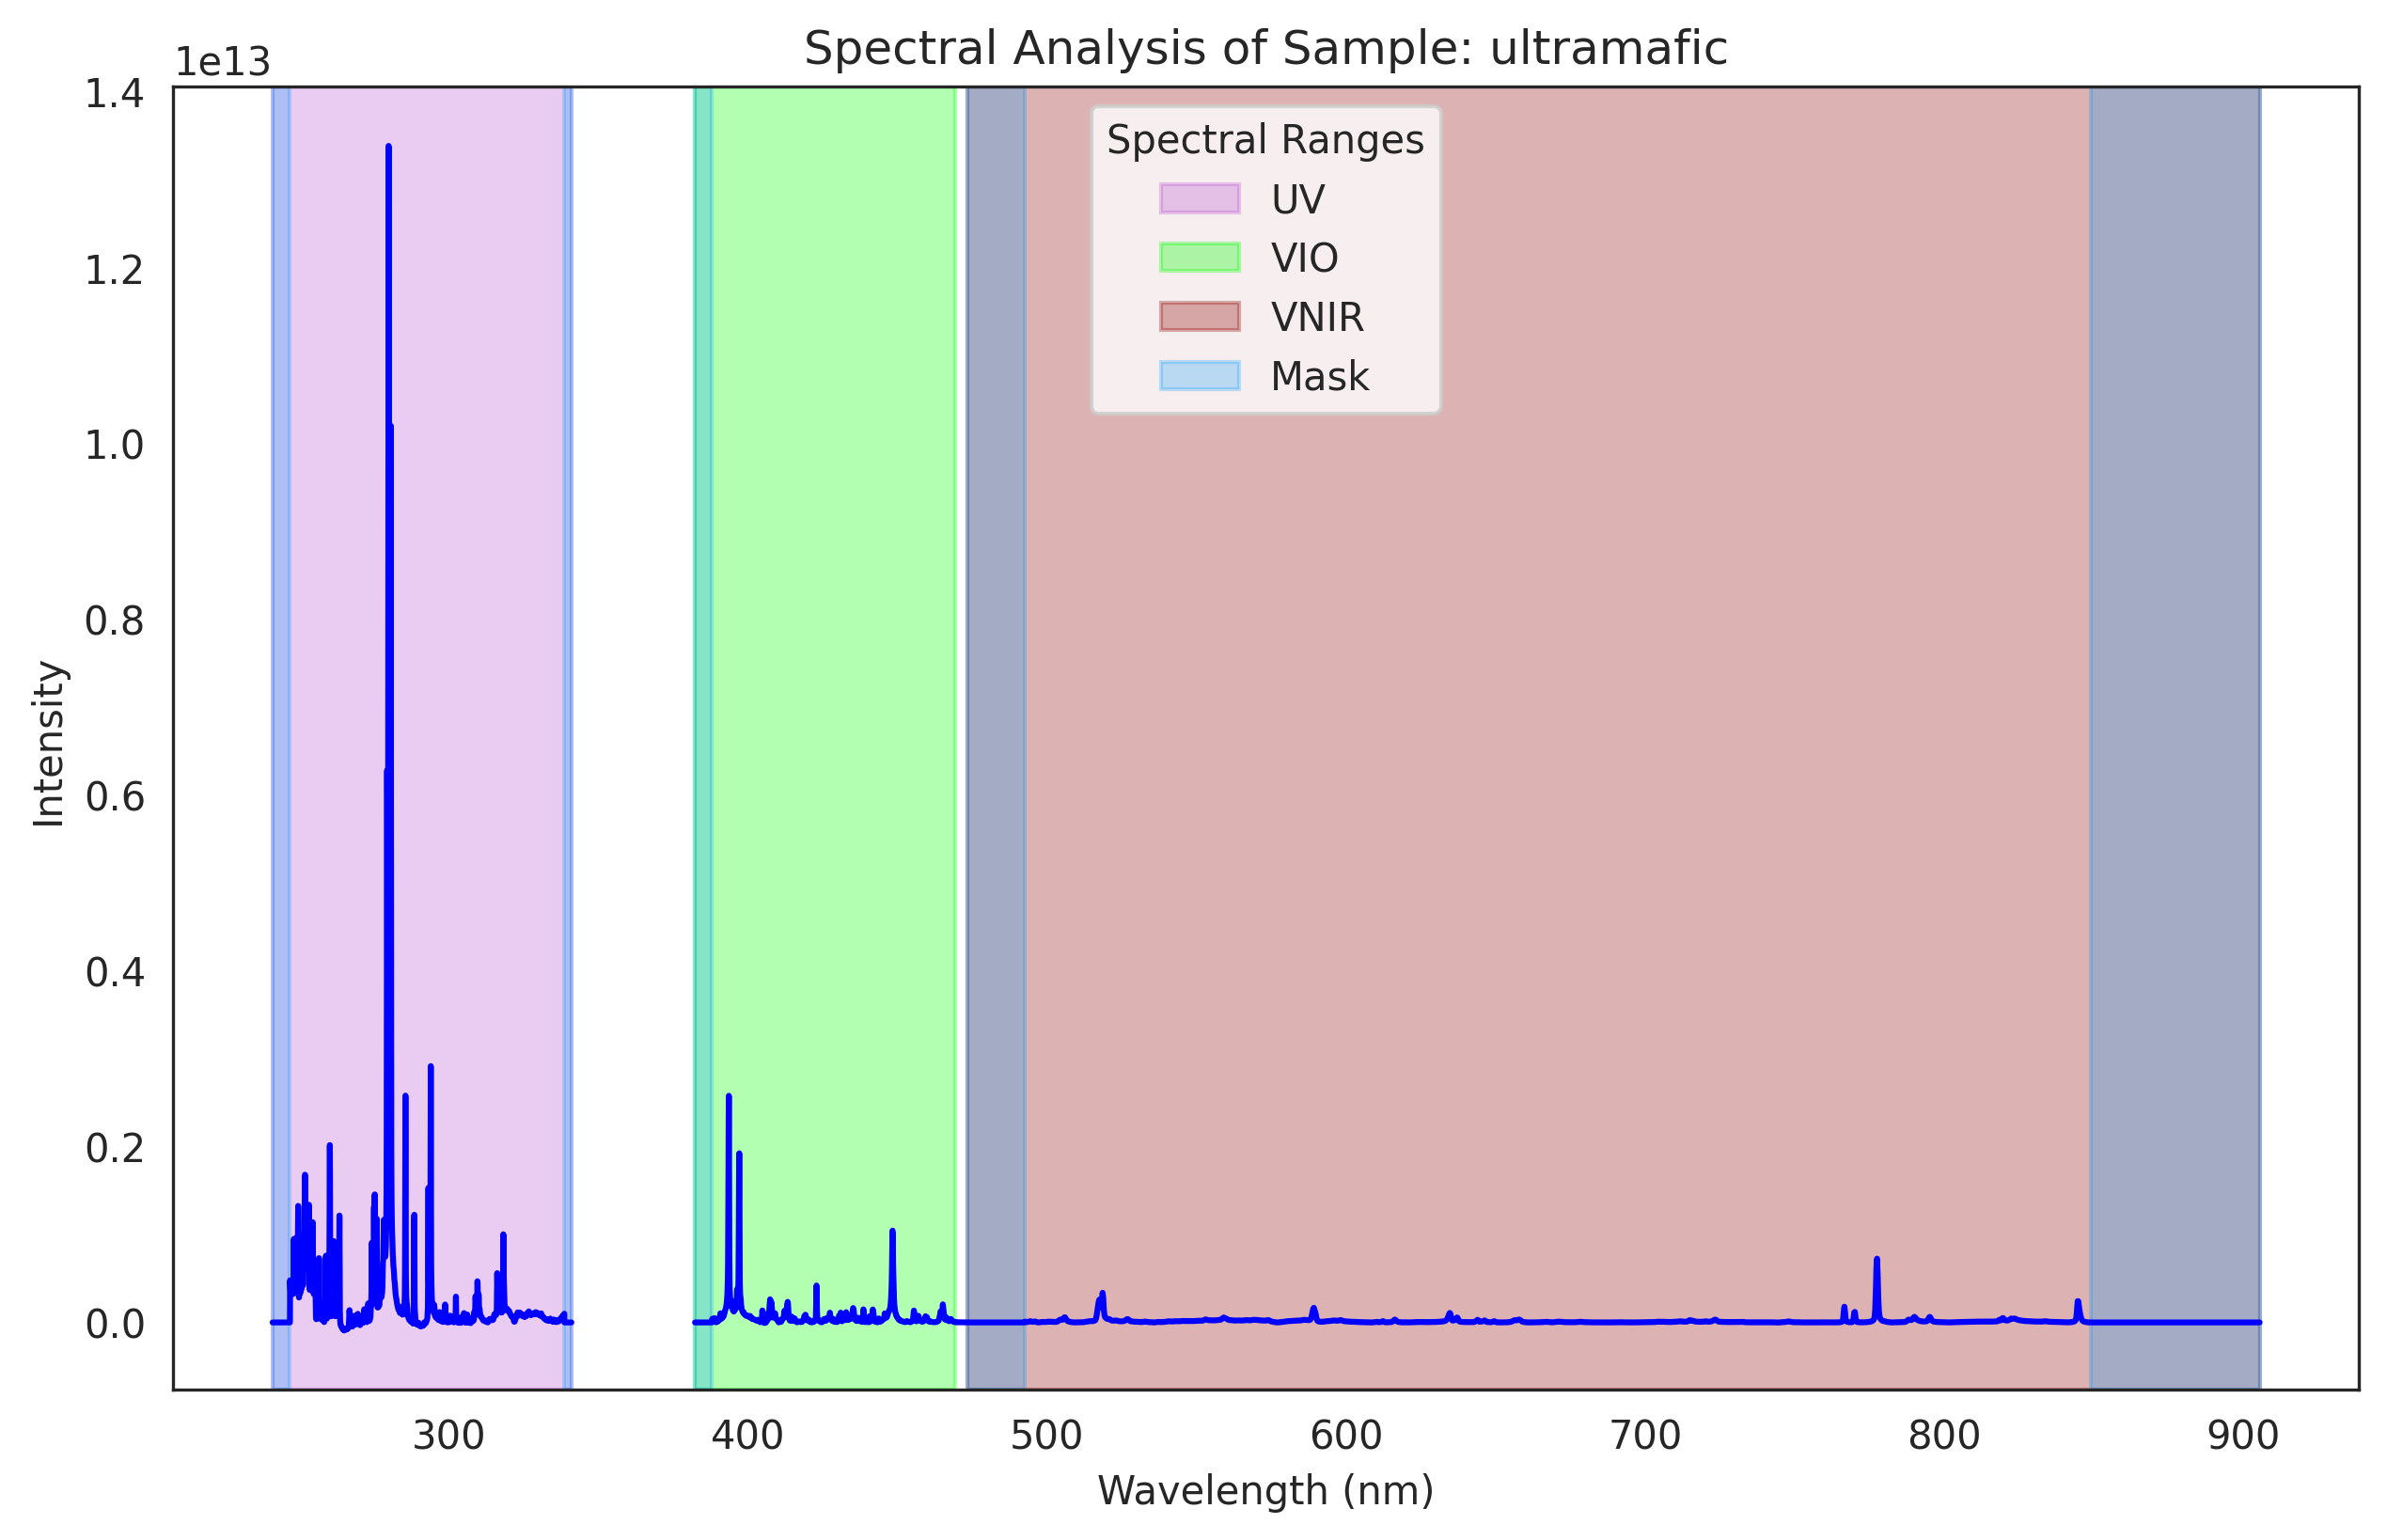
\includegraphics[width=0.5\textwidth]{images/spectral_plot.png}
	\caption{Spectral plot of the \gls{ccs} data for the \textit{ultramafic} sample. The wavelengths represent the spectral channels.}
	\label{fig:spectral_plot}
\end{figure}

Norm 3 can be understood as follows: for each sample, we consider the data from each spectrometer separately. Within each spectrometer, we divide the intensity of each channel by the sum of all channel intensities for that spectrometer. This process is applied for all three spectrometers, resulting in normalized data that preserves the relative intensities within each spectrometer while allowing for comparisons across different samples.

Formally, Norm 3 is defined as

\begin{equation}
	\tilde{X}_{i,j}^{(\gamma)} = \frac{X_{i,j}^{(\gamma)}}{\sum_{j=1}^{N} X_{i,j}^{(\gamma)}},
\end{equation}

where

\begin{itemize}
	\item $\tilde{X}_{i,j}^{(\gamma)}$ is the normalized wavelength intensity for the $i$-th sample in the $j$-th channel on the $\gamma$-th spectrometer with $\gamma \in \{1, 2, 3\}$,
	\item $X_{i,j}^{(\gamma)}$ is the original wavelength intensity for the $i$-th sample in the $j$-th channel on the $\gamma$-th spectrometer,
	\item $N = 2048$ is the number of channels in each spectrometer, and
\end{itemize}

This normalization method results in a total of $3N = 6144$ normalized features for each sample, as each of the three spectrometers contributes 2048 channels.

\subsection{Overview of Core Models}
In this section, we provide an overview and definitions of \gls{pls}, primarily based on the methodologies described by \citet{James2023AnIS}.
These models form the basis of the final architecture of our proposed pipeline, detailed further in Section~\ref{sec:methodology}.

\subsubsection{PLS}
To understand \gls{pls}, it is essential to first understand \gls{pca} and \gls{pcr}.

\gls{pca} is a dimensionality reduction technique that transforms a set of possibly correlated variables into a smaller set of uncorrelated variables called \textit{principal components}.
First, the data matrix $\mathbf{X}$ is centered by subtracting the mean of each variable to ensure that the data is centered at the origin:

$$
\mathbf{\bar{X}} = \mathbf{X} - \mathbf{\mu},
$$

where $\mathbf{\bar{X}}$ is the centered data matrix and $\mathbf{\mu}$ is the mean of each variable.

The covariance matrix of the centered data is then computed:

$$
\mathbf{C} = \frac{1}{n-1} \mathbf{\bar{X}}^T \mathbf{\bar{X}},
$$

where $n$ is the number of samples.

Then, the covariance matrix $C$ is decomposed into its eigenvectors $\mathbf{V}$ and eigenvalues $\mathbf{D}$:

$$
\mathbf{C} = \mathbf{V} \mathbf{D} \mathbf{V}^T,
$$

where matrix $\mathbf{V}$ contains the eigenvectors of $\mathbf{C}$ and represents the principal component loadings.
These loadings indicate the directions of maximum variance in $\mathbf{X}$.
The matrix $\mathbf{D}$ is diagonal and holds the eigenvalues, each of which quantifies the variance captured by its corresponding loading.

These components are the scores $\mathbf{T}$, calculated as follows:

$$
\mathbf{T} = \mathbf{\bar{X}} \mathbf{V}_n,
$$

where $\mathbf{V}_n$ includes only the top $n$ eigenvectors.
The scores $\mathbf{T}$ are the new, uncorrelated features that reduce the dimensionality of the original data, capturing the most significant patterns and trends.

Finally, the original data points are projected onto the space defined by the top $n$ principal components, which transforms $X$ into a lower-dimensional representation:

$$
\mathbf{X}_{\text{reduced}} = \mathbf{\bar{X}} \mathbf{V}_n,
$$

where $\mathbf{V}_n$ is the matrix that only contains the top $n$ eigenvectors.

\gls{pcr} extends \gls{pca} in the context of regression analysis.
First, \gls{pca} is applied to the dataset $\mathbf{X}$, transforming it into a set of uncorrelated variables, the principal components.
These components, represented by scores $\mathbf{T}$, are derived from the eigenvectors $\mathbf{V}_n$ with the highest variances.

In \gls{pcr}, the dataset $\mathbf{X}$ is decomposed using PCA as:

$$
\mathbf{X} = \mathbf{TV}^T + \mathbf{E},
$$

where $\mathbf{T}$ represents the scores, and $\mathbf{V}$ represents the loadings.
\gls{pcr} utilizes these scores $\mathbf{T}$ in a linear regression model to predict the target variable $\mathbf{y}$:

$$
\mathbf{y} = \mathbf{Tb} + \mathbf{e},
$$

where $\mathbf{b}$ are the regression coefficients correlating $\mathbf{T}$ to $\mathbf{y}$, and $\mathbf{e}$ is the vector of residuals, capturing the prediction errors.

However, one drawback of \gls{pcr} is that it does not consider the target in the decomposition of the features and therefore assumes that smaller components have a weaker correlation with the target than the larger ones.
This assumption does not always hold, which is what \gls{pls} aims to address.

\gls{pls} uses an iterative method to identify components that maximize the covariance between the features and the target.
These components, $Z$, are linear combinations of the original features, $X_j$, weighted by coefficients, $\phi_j$, which are specifically calculated to reflect this covariance.
The formula for each component is expressed as:

$$
    Z = \sum_{j=1}^{p} \phi_j X_j,
$$

where $Z$ represents the component, $X_j$ is the $j$-th feature, and $\phi_j$ is the weight for the $j$-th feature.
The weights, $\phi_j$, are determined by the formula:

$$
    \phi_j = \frac{\text{cov}(X_j, Y)}{\text{var}(X_j)}.
$$

To refine the model iteratively, PLS uses the residuals from the previous components to calculate the next component.
The $m$-th component, for example, is derived from the residuals of the previous $m-1$ components:

$$
    Z_m = \sum_{j=1}^{p} \phi_{jm} \hat{X}_{j, m-1}.
$$

The components are then used to predict the target variable by fitting a linear model via least squares regression.

\subsubsection{Gradient Boosting Regression}\label{sec:gradientboost}
Gradient boosting is an approach that is builds on a set of simpler concepts.
It incorporates the idea of ensemble learning, with decision trees and boosting as its core components. 

Ensemble learning is a machine learning technique where mulitple models, known as \textit{weak learners}, are combined to produce more accurate predictions.
Mathematically, ensemble learning can be defined as combining the predictions of $M$ weak learners to form a final prediction $\hat{y}$, such that:
\begin{equation}
    \hat{y} = \sum_{m=1}^{M} \alpha_m \hat{y}_m
\end{equation}
where $\hat{y}_m$ is the prediction of the $m$-th weak learner and $\alpha_m$ is the weight assigned to the $m$-th weak learner.
Although various options exist for weak learners, decision trees are commonly used and have been selected for this study.

The basic approach to decision trees involves partitioning the data into subsets based on feature values, with the goal of creating groups where the data points are more similar to each other in their predicted outcomes. 
This similarity, or homogeneity, is described in terms of impurity, which is a measure of how mixed the data points are in a given region. 
This is achieved through recursive binary splitting, where the dataset is divided into two regions based on the value of one of the predictors. 
The aim at each step is to select the predictor and the split point that result in the greatest reduction in impurity.

Impurity, in the context of regression trees, is measured using the \gls{rss}.
Mathematically, for any predictor $X_j$ and split point $s$, the data is divided into two regions $R1$ and $R2$ defined as:
$$
\begin{aligned}
    R1(j, s) &= \{X | X_j < s\} \\
    R2(j, s) &= \{X | X_j \geq s\}
\end{aligned}
$$

The goal is to find the values of $j$ and $s$ that minimize the RSS, which is calculated as:
$$
\sum_{i: x_i \in R1(j, s)} (y_i - \hat{y}_{R1})^2 + \sum_{i: x_i \in R2(j, s)} (y_i - \hat{y}_{R2})^2
$$

where $\hat{y}_{R1}$ and $\hat{y}_{R2}$ are the mean responses for the training observations in regions $R1$ and $R2$, respectively, $y_i$ is the response for the $i$-th observation and $x_i$ is the predictor value for the $i$-th observation. 

Once the optimal splits are identified, the tree is constructed by repeating this process for each subset until a stopping criterion, such as a minimum number of observations per node, is met. 
The final model consists of splits that create distinct regions, each with a predicted response value based on the mean of the training observations in that region.

This method ensures each region is more homogeneous with respect to the target variable, effectively reducing impurity and making the data points within each region more similar.

The predictions resulting from the decision trees can then be improved by growing the trees sequentially, with each new tree correcting the errors of the previous ones.
This technique is referred to as \textit{Gradient Boosting}.
A usual feature of boosted trees, is that each tree is typically small, with few terminal nodes.
The small size of the trees and small number of terminal nodes prevents the model from making large adjustments based on a single tree's predictions.
It also ensures that each tree makes small and simple error corrections, such that each step refines the model's performance more reliably.
Finally, small trees have the property of high bias, meaning that they are unable to capture complex relationships in the data and low variance.
By combining multiple small trees, the model can capture complex relationships while maintaining a low variance.

As implied, the model is constructed iteratively by adding trees to correct the residuals of the previous trees. Mathematically, the final model is given by:
\begin{equation}
    \hat{f}(x) = \sum_{b=1}^{B} \lambda \hat{f}_b(x) 
\label{eq:boosted_tree}
\end{equation}

where $\hat{f}_b(x)$ is the prediction of the $b$-th tree, $B$ is the number of trees in the model and $\lambda$ is the learning rate.
This model is obtained by first setting the initial prediction $\hat{f}_0(x) = 0$ and $r_i = y_i$ for all $i$ in the training set.Then the predictions are updated at each iteration $b$ as: 

$$
\hat{f}(x) \leftarrow \hat{f}(x) + \lambda \hat{f}_b(x)
$$

where $\hat{f}_b(x)$ is the prediction of the $b$-th tree and $\lambda$ is the learning rate. 
The residuals, which represent the errors to be corrected by the next tree, are updated as:

$$
r_i \leftarrow y_i - \hat{f}(x)
$$

At each step, a new regression tree $\hat{f}_b(x)$ is trained on these residuals.
That is, each tree is learning to predict how much the previous model was wrong.
The process of training a weak learner to predict the residuals and using its predictions to update the model is repeated for $B$ iterations, resulting in the final model in equation~\ref{eq:boosted_tree}.
The process of training a weak learner to predict the residuals and using its predictions to update the model is repeated for $B$ iterations, resulting in the final model in equation~\ref{eq:boosted_tree}. 
Each tree is trained to target the negative gradient of the loss function, defined as:
$$
    \nabla L = y - \hat{y}
$$ 
which directs the model's adjustments in the steepest descent direction to efficiently reduce errors.
A commonly used loss function for \gls{gbr} is the squared error: 
$$ 
    L = \frac{1}{2}(y - \hat{y})^2
$$
favored for its continuous and differentiable nature which facilitates the gradient computation and ensures stable optimization paths. 



\subsubsection{Gradient Boosting Regression}\label{sec:gradientboost}
Gradient boosting builds on simpler concepts and incorporates the idea of ensemble learning, with decision trees and boosting as its core components.

Ensemble learning is a technique in machine learning where multiple models, known as \textit{weak learners}, are combined to produce more accurate predictions.
Mathematically, ensemble learning can be defined as combining the predictions of $M$ weak learners to form a final prediction $\hat{y}$, such that:
\begin{equation}
    \hat{y} = \sum_{m=1}^{M} \alpha_m \hat{y}_m
\end{equation}
where $\hat{y}_m$ is the prediction of the $m$-th weak learner and $\alpha_m$ is the weight assigned to the $m$-th weak learner.
Although various options exist for weak learners, decision trees are commonly used and have been selected for this study.

Decision trees partition the data into subsets based on feature values, aiming to create groups where the data points are more similar in their predicted outcomes. 
This similarity, or homogeneity, is measured in terms of impurity, which is a measure of how mixed the data points are within a region. 
This is achieved through recursive binary splitting, dividing the dataset into two regions based on the value of a predictor. 
The goal at each step is to select the predictor and the split point that result in the greatest reduction in impurity.

Impurity, in the context of decision trees, is measured using the residual sum of squares (RSS). For any predictor $X_j$ and split point $s$, the data is divided into two regions $R1$ and $R2$ defined as:
$$
\begin{aligned}
    R1(j, s) &= \{X | X_j < s\} \\
    R2(j, s) &= \{X | X_j \geq s\}
\end{aligned}
$$
The goal is to find the values of $j$ and $s$ that minimize the RSS, calculated as:
$$
    \sum_{i: x_i \in R1(j, s)} (y_i - \hat{y}_{R1})^2 + \sum_{i: x_i \in R2(j, s)} (y_i - \hat{y}_{R2})^2
$$
where $\hat{y}_{R1}$ and $\hat{y}_{R2}$ are the mean responses for the training observations in regions $R1$ and $R2$, respectively.

Once optimal splits are identified, the tree is constructed by repeating this process for each subset until a stopping criterion is met. 
The final model consists of splits that create distinct regions, each with a predicted response value based on the mean of the observations in that region.

The method ensures that each region is more homogeneous with respect to the target variable, effectively reducing impurity and making the data points within each region more similar.

The predictions from the decision trees can then be improved by growing the trees sequentially, with each new tree correcting the errors of the previous ones. 
This technique is referred to as \textit{Gradient Boosting}. 
Each tree is small, with few terminal nodes, preventing large adjustments based on a single tree's predictions. 
It also ensures that each tree makes small and simple error corrections, such that each step refines the model's performance more reliably.
Finally, small trees have the property of high bias, meaning that they are unable to capture complex relationships in the data and low variance.
By combining multiple small trees, the model can capture complex relationships while maintaining a low variance.

The model is constructed iteratively by adding trees to correct the residuals of the previous trees. 
Initially, the prediction is set as $\hat{f}_0(x) = 0$ and residuals as $r_i = y_i$ for all $i$ in the training set. 
At each iteration $b$, predictions are updated as:
$$
    \hat{f}(x) = \hat{f}(x) + \lambda \hat{f}_b(x)
$$
where $\hat{f}_b(x)$ is the prediction of the $b$-th tree and $\lambda$ is the learning rate. Residuals, representing the errors to be corrected by the next tree, are updated as:
$$
    r_i = y_i - \hat{f}(x)
$$
Each tree is then trained on these updated residuals. This process of fitting a weak learner to predict the residuals and using its predictions to update the model is repeated for $B$ iterations, culminating in the final model:
$$
    \hat{f}(x) = \sum_{b=1}^{B} \lambda \hat{f}_b(x) 
$$
This final formulation effectively reduces errors by moving in the direction of the steepest descent as dictated by the gradient of the loss function. The commonly used squared error loss function is:
$$
L = \frac{1}{2}(y - \hat{y})^2
$$
which is continuous and differentiable, facilitating the computation of the gradient and ensuring stable optimization paths. The gradient, defined as:
$$
    \nabla L = y - \hat{f}(x),
$$
guides the model adjustments to efficiently reduce errors. 
The learning rate $\lambda$ moderates the size of these adjustments, helping to maintain stability and prevent overfitting as the model iteratively fits to the residual errors.


1. Introduction to Ensemble Methods
    * Brief Introduction to Machine Learning: Supervised learning and prediction.
    * Ensemble Methods: Combining multiple models for better performance.
2. Decision Trees
    * Concept: Explain the basic idea of decision trees.
    * Pros and Cons: Advantages (interpretability, simplicity) and disadvantages (overfitting, instability).
3. Bagging and Boosting
    * Bagging: Mention briefly how bagging (Bootstrap Aggregating) works with decision trees (e.g., Random Forests).
    * Boosting: Introduce boosting, focusing on the idea of sequentially training models to correct previous errors.
4. Gradient Boosting
    * Concept: Explain gradient boosting as a method to minimize a loss function using gradients.
    * Training Process: Describe the iterative process of adding models to correct residuals.
5. Gradient Boosting Regressor
    * Implementation: Mention sklearn's Gradient Boosting Regressor, which uses decision trees as base learners.
    * Advantages: Robust performance and ability to handle complex relationships
    * Slow learner - Advantageous